\documentclass{article}

\usepackage{project_440_540}
% Please submit it as is here, with line numbers.
% If you'd like a "less draft"-looking version for your website or something after:
%     \usepackage[final]{project_440_540}   % keeps the footer but kills line numbers,
%     \usepackage[preprint]{project_440_540}   % removes both


\usepackage[utf8]{inputenc} % allow utf-8 input
\usepackage[T1]{fontenc}    % use 8-bit T1 fonts

\usepackage[USenglish]{babel}  % there's a "canadian" option, but it's an alias for USenglish,
                               % and for some reason it makes csqoutes behave differently...
\usepackage{csquotes}       % smarter handling of quotes (used by biblatex)

\usepackage{booktabs}       % professional-quality tables
\usepackage{amsfonts}       % blackboard math symbols
\usepackage{nicefrac}       % compact symbols for 1/2, etc.
\usepackage{microtype}      % microtypography
\usepackage{xcolor}         % colors
\usepackage{hyperref}       % hyperlinks
\usepackage{url}            % simple URL typesetting
\usepackage{tikz}


% I recommend the biblatex package.
% If you hate it for some reason, though, you can use natbib instead:
% comment out this block and uncomment the next one.

\usepackage[style=authoryear,maxbibnames=30]{biblatex}
\addbibresource{refs.bib}
\renewbibmacro{in:}{}  % drops a silly "In:" from biblatex format
\let\citet\textcite    % I do this alias because I/others find it more familiar, idk.
\let\citep\parencite   % biblatex also has a natbib option to make these,
                       % but makes other changes I don't care about too.
\usepackage{bibentry}
%\usepackage{natbib}



\usepackage[capitalize,noabbrev]{cleveref}


\title{Implementing Complex Valued Neural Networks}


% The \author macro works with any number of authors. There are two commands
% used to separate the names and addresses of multiple authors: \And and \AND.
%
% Using \And between authors leaves it to LaTeX to determine where to break the
% lines. Using \AND forces a line break at that point. So, if LaTeX puts 3 of 4
% authors names on the first line, and the last on the second line, try using
% \AND instead of \And before the third author name.

\author{%
  Alexander MacFarlane\\
  \texttt{djmacfarlanez@gmail.com}
}

\begin{document}
\maketitle


\begin{abstract}
\end{abstract}
\section{Introduction}
Complex valued neural networks (CVNNs) offer several potential advantages over real valued neural networks (RVNNs). By incorporating both phase and magnitude in each value, CVNNs allow for a richer representation of data. This increased information content in each input and parameter can lead to a reduction in the number of parameters, subsequently lowering the likelihood of exploding and vanishing gradients while also reducing the need for regularization. Furthermore, some types of data are naturally suited for representation using complex numbers.

CVNNs hold great promise in domains where complex values are already extensively utilized, such as quantum computing and signal processing. Outputs from Fourier transforms and other complex representations can be directly fed into the network, eliminating the need to separate or remove information from each value as required with RVNNs. Additionally, certain complex transforms and filters can be applied to images, thereby reducing the need for convolutions in image classification tasks\footnote{See \cite{ko2022coshnet}}.

Despite these advantages, many popular neural network frameworks, such as PyTorch and Keras with TensorFlow, offer limited support for complex valued neural networks by default. Nevertheless, TensorFlow does provide support for complex tensors, which enables the implementation of CVNNs by defining custom layers. In this project, we take advantage of this functionality to explore the potential of CVNNs further.


\section{Related Works}
\begin{center}\textbf{\fullcite{CVNN_book}}\end{center}
This book provides an overview of complex valued neural networks and some applications. Much of the implementation is based on concepts from this author's works.\\ \\
\begin{center}\textbf{\fullcite{ko2022coshnet}}\end{center}
In this paper they explore shearlets and CVNNs in image processing to reduce the need for convolution, increase efficiency and improve performance. This is an excellent demonstration that CVNNs are worth investigating. \\ \\
\begin{center}\textbf{\fullcite{biocvnn}}\end{center}
The primary motivation for this project was the potential of CVNNs to more accurately approximate biological networks. The paper investigates CVNNs, which are designed to be more similar to biological neural networks than their real-valued neural network (RVNN) counterparts, demonstrating superior performance in certain tasks. However, the paper's main drawback lies in its reliance on gradient descent as a training method, as this is likely an unrealistic learning mechanism for biological systems \citep{hintonforwardforward}.

\section{Description}

\section{Experiments}
\subsection{MNIST}
To test the implementation we do a trial run on MNIST data set to verify the implementation is functioning. For the real neural network we use 32 filter 4 by 4 kernels with softmax output layer. The complex network has 16 filters of 4 by 4 kernels to halve the number of parameters. CVNNs do not offer much benefit in a simple case like this, but is a convenient test set.
\begin{figure}[h]
  \centering
  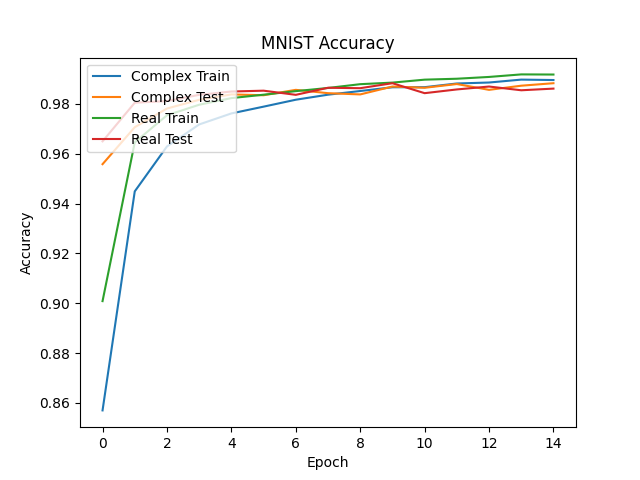
\includegraphics[width=0.6\textwidth]{../figs/combined.png}
  \caption{As expected we get similar performance.}
\end{figure}

%\printbibliography
\end{document}
